\documentclass[12pt,a4paper]{article}

\usepackage{float}
\usepackage{caption}
\usepackage{amsmath}
\usepackage{amsfonts}
\usepackage{amssymb}
\usepackage{graphicx}
\usepackage{xcolor}
\usepackage{geometry}
\usepackage{braket}

\geometry{
	top=0.6in, % Top margin
	bottom=0.6in, % Bottom margin
	left=0.75in, % Left margin
	right=0.75in, % Right margin
}

\newcommand{\ua}{\ket{\uparrow}}
\newcommand{\da}{\ket{\downarrow}}
\newcommand\nm[1]{\lVert #1 \rVert}


\title{Tricky stuff}
\author{Jan Engler}
\date{Last change: \today}

\begin{document}
\maketitle
\tableofcontents

\subsection{Measurable set that is not borel}
\par Let $\mathcal{C}\subset [0,1]$ be Cantor set, $c\colon[0,1]\to[0,1]$ be cantor function defined by
\begin{align*}
	c &= \frac{1}{2} \text{ on } \left[\frac{1}{3},\frac{2}{3}\right] \\
	c &= \frac{1}{4} \text{ on } \left[\frac{1}{9},\frac{2}{9}\right], \ c=\frac{3}{4} \text{ on } \left[\frac{7}{9},\frac{8}{9}\right] \\
	  &\ \ \vdots \\
	c\left(\sum_{n\in \mathbb{N}}\frac{2a_n}{3^{n}}\right) &= \sum_{n\in \mathbb{N}}\frac{a_n}{2^n} \ \ \forall \{a_n\}_{n\in \mathbb{N}}, \ a_n\in\{0,1\} \\
	c(x) &= \sup_{y\leq x}c(y) \text{ for } x\in [0,1]\setminus \mathcal{C}
\end{align*}
Then $c$ is continuous, surjective and nondecreasing. Therefore
\begin{equation*}
  \psi(x) = c(x)+x
\end{equation*}
is continuous, increasing and bijective $[0,1]\to[0,2].$ Since
\begin{align*}
	[0,1]\setminus\mathcal{C} &= \bigcup_{n\in \mathbb{N}}(a_n,b_n) \text{ where } (a_n,b_n) \text{ are intervals} \\
	\lambda\left(\psi\left(a_n,b_n\right)\right) &= \lambda(c(a_n)+a_n,c(b_n)+b_n)=\lambda(c|_{A_n}+a_n,c|_{A_n}+b_n)=\lambda(a_n,b_n) \\
	\lambda(\psi([0,1]\setminus \mathcal{C}))&=\lambda([0,1]\setminus \mathcal{C})=1 \\
	\lambda(\psi(\mathcal{C})) &= \lambda([])
\end{align*}
\par On the other hand, the completion of Borel sigma algebra is easily seen to be Lebesque sigma algebra:
\par Denote $\mathcal{B}$ Borel algebra, $\mathcal{L}$ Lebesque algebra, $\overline{\mathcal{B}}^\lambda$ the completion of $\mathcal{B}$ w.r.t. Lebesque measure $\lambda,$ $G_\delta$ to be set of countable intersections of open sets ("$G_\delta$" sets). Clearly $\overline{\mathcal{B}}^\lambda\subset \mathcal{L}.$ To prove the other inclusion, choose arbitrary $A\in \mathcal{L}.$ Then $\exists B\in G_\delta\colon A\subset B, \ \lambda(B\setminus A)=0,$ so
\begin{equation*}
	A = \underbrace{B}_{\in \mathcal{B}}\setminus \underbrace{(B\setminus A)}_{\in \overline{\mathcal{B}}^\lambda, \text{ since } \lambda(B\setminus A)=0}\in \overline{\mathcal{B}}^\lambda
\end{equation*}


\subsection{Hölder continuous function not absolutely continuous}
Let $c$ be the cantor function and $c_k$ be defined by
\begin{align*}
	&c_k\left(\sum_{n=1}^k \frac{2a_n}{3^n}\right)=\sum_{n=1}^k \frac{a_n}{2^n} \ \ \forall \{a_n\}_{n=0}^k, a_n\in \{0,1\} \\
	&c_k \text{ is piecewise linear on } [0,1] \\
	&c_k(0)=0, c_k(1)=1
\end{align*}
Then 
\begin{itemize}
	\item \nm{c-c_k}_{\infty} = 2^{-k}
	\item $c_k$ is Lipschitz with constant $\displaystyle\left(\frac{3}{2}\right)^k$ (think about the slope of steepest line)
\end{itemize}
So for $x,y \in [0,1]$
\begin{align*}
	|c(x)-c(x)|&\leq \nm{c-c_k}_{\infty} + |c_k(x)-c_k(y)| + \nm{c-c_k}_{\infty}  \\
			   &\leq 2\cdot 2^{-k} + \left(\frac{3}{2}\right)^k|x-y|
\end{align*}
Choose $k\in \mathbb{N}$ such that $3^{-k-1}\leq |x-y| < 3^{-k},$ then
\begin{equation*}
	|c(x)-c(y)|\leq 3\cdot 2^{-k} = 6\cdot 2^{-k-1} = 6\cdot 3^{-(k-1)\cdot \log_32} < 6\cdot |x-y|^{\log_32}
\end{equation*}
So the cantor function is $\log_32$-Hölder continuous. \\
Let $\epsilon>0$. Since $c$ is locally constant on $[0,1]\setminus \mathcal{C},$ which is a countable union of open intervals with measure one, by continuity of measure we can choose $x_1, ..., x_n, y_1, ..., y_n\in [0,1], x_k<y_k$ (in fact they will be endpoints of form $\frac{l}{3^n}, l,n\in \mathbb{N}$) such that
\begin{equation*}
	\sum_{k=1}^n |y_k-x_k| > 1-\epsilon \ \ \text{ and c is constant on intervals} \ \ (x_k,y_k)  
\end{equation*}
Since c is constant on big set, and $c(0)=0, c(1)=1,$ it must grow fast on a small set:
\begin{align*}
	|x_1-0| + \sum_{k=1}^{n-1} |x_{k+1}-y_{k}| + |1-y_n| = 1-\sum_{k=1}^n |y_k-x_k| &< \epsilon \\
	\text{BUT} \ \ c(x_1)-c(0) + \sum_{k=1}^{n-1}(c(x_{k+1})-c(y_k))+c(1)-c(y_n) = 1-\sum_{k=1}^n(c(y_k)-c(x_k))&=1 
\end{align*}
so $c$ is not $AC[0,1].$ A shorter proof might use characterization $AC[0,1]=W^{1,1}(0,1),$ since $c$ has classical derivative zero almost everywhere, but certainly
\begin{equation*}
	c(0)+\int_{0}^1 c'(x)dx = 0+\int_{0}^1 0\ dx = 0 \neq c(1)
\end{equation*}
In fact, $c\in BV[0,1]\setminus AC[0,1]$ and it's Lebesque-Stieltjes measure is singular nonatomic with respect to the Lebesque measure on $[0,1].$ 

\subsection{Hopf fibration, dirac belt}

\begin{equation*}
	S^{1} \to S^{3} \cong B_{1,\mathbb{C}^2}(0) \to S^{2} \cong \mathbb{PC}^{1}
\end{equation*}
Hilbert space for two-state system is
\begin{equation*}
	\mathcal{H}=\mathbb{C}^2 = \mathbb{C}\ua \oplus \mathbb{C}\da
\end{equation*}
When we mod out the norm, we are left with $B_{1,\mathbb{C}^2}(0) \cong S^{3}$ and when we mod out the phase, we are left with $\frac{S^{3}}{S^{1}}\cong S^{2}.$ Quantum evolution happens on $S^{3}$ and state space is $S^{2}=\mathbb{P}(\mathcal{H}).$ 

Below we use pauli matrices
\begin{equation*}
  \sigma_x =
  \begin{pmatrix}
	  0 & 1 \\ 1 & 0
  \end{pmatrix}, \ \ 
  \sigma_y = 
  \begin{pmatrix}
	  0 & -i \\ i & 0
  \end{pmatrix}, \ \
  \sigma_z = 
  \begin{pmatrix}
	  1 & 0 \\ 0 & -1
  \end{pmatrix}, \ \ 
  \vec{\sigma} = 
  \begin{pmatrix}
    \sigma_x \\ \sigma_y \\ \sigma_z
  \end{pmatrix}
\end{equation*}

The Hopf fibration is the map which sends spinors (elements of $S^3$) to the expectation values of spin in the $x,y,z$ directions:
\begin{align*}
	\langle \bullet | \vec{\sigma} | \bullet \rangle\colon S^3 &\to S^2 \\
	\alpha\ua+\beta\da = \ket{\psi} &\mapsto \bra{\psi}\vec{\sigma}\ket{\psi} = 
	\begin{pmatrix}
\langle \sigma_x \rangle _{\psi} \\
\langle \sigma_y \rangle _{\psi} \\
\langle \sigma_x \rangle _{\psi} \\
\end{pmatrix} \\
\text{or: } 
\begin{pmatrix}
	\alpha \\
	\beta
\end{pmatrix}
&\mapsto 
\begin{pmatrix}
	\alpha \bar{\beta}+\beta \bar{\alpha} \\
	i(\alpha \bar{\beta}-\beta \bar{\alpha}) \\
	|\alpha|^2 - |\beta|^2
\end{pmatrix}
\end{align*}

Generally, given a smooth manifold $M$, a principal $U(1)$-bundle is a fiber bundle $p\colon E\to M$ with a group action $U(1)\times E \to E$ such that $\forall e\in E, g\in G:\ e\in p^{-1}(x) \Rightarrow  g\cdot e \in p^{-1}(x)$ and the action on each fiber is free and transitive. In our case $M=S^{2}.$

%TODO: ADD DIRAC BELT

\subsection{Examples of adjunctions}
$Unif$ is category of uniform spaces and uniformly cts functions, $CUnif_{T2}$ is category of complete hausdorff uniform spaces, $\hat{A}$ is completion of $A$. 
\begin{equation*}
	Hom_{Unif}(A,Y) \cong Hom_{CUnif_{T2}}(\hat{A} ,Y)
\end{equation*}

\subsection{Homeomorphism doesn't preserve completeness}
Completeness is not a topological invariant. The spaces $(0,1),\ \mathbb{R}$ with Euclidean topology are homeomorphic via
\begin{equation*}
  h\colon \mathbb{R} \to (0,1), \ \ h(x) = \frac{\tanh(x)+1}{2}
\end{equation*}
$\mathbb{R}$ is complete, $(0,1)$ is not. 

\subsection{Frechet space that is not normable}
Consider $L^1_{loc}(\mathbb{R}^d)$ given the F topology generated by seminorms
\begin{equation*}
	|f|_n = \int_{\nm{x}\leq n}|f(y)|dy
\end{equation*}
Suppose there is a norm $\nm{\bullet}$ generating the same topology. Then $\exists C>0, C_n>0, n\in \mathbb{N}$ such that
\begin{align}
	\nm{\bullet}&\leq C|\!\bullet\!|_N, \\
	|\!\bullet\!|_n &\leq C_n \nm{\bullet}
\end{align}
from this we get $|\!\bullet\!|_{N+1}\leq C_{N+1}C|\!\bullet\!|_N$, which is clearly wrong for the function $f=\chi_{\{N<\nm{x}<N+1\}}.$
\par To prove (1), for contradiction, assume
\begin{equation*}
	\forall n,k\in \mathbb{N} \ \exists \phi_{n,k}\in L^{1}_{loc}: \nm{\phi_{n,k}}>n|\phi_{n,k}|_k
\end{equation*}
define $\psi_n = \displaystyle\frac{\phi_{n,n}}{n|\phi_{n,n}|_n},$ then 
\begin{equation*}
  \forall l\in \mathbb{N}, n\geq l: |\psi_n|_l \leq |\psi_n|_n = \frac{1}{n} \to 0 \ \ \ \ n\to \infty
\end{equation*}
so $\psi_n \to 0$ in $L^1_{loc}$ but $\nm{\psi_n}>1,$ contradiction. Generally, for any Frechet space $X$ where the seminorms are nondecreasing, the inequalities (1) and (2) hold, so if we can find elements $x\in X$ such that $|x|_{N+1}$ can be arbitrarily large and $|x|_N$ arbitrarily small, the space is nor normable.
\par For $C^\infty_0[0,1]$ where topology is generated by $|f|_n = \sup_{k\leq n}\nm{f^{(k)}}_\infty$, the element $f(x)=\frac{1}{n^N}\sin(nx)$ ($n$ large) has small $|\bullet|_{N-1}$ but large $|\bullet|_N.$

\subsection{Banach space with no preduals}
Suppose $X^{*}=L^1(0,1).$ Then by Banach-Alaoglu, $B_X = \{f\in L^1(0,1)\colon \nm{f}\leq 1\}$ is $w^{*}-compact$ convex, so by Krein-Milman $B_X=\overline{\text{aconv}}\ \text{ext } B_X$. But there are no extreme points of $B_X:$
\par Suppose $f\in B_X$ is extreme. Since $\int_0^x|f(t)|dt$ is continuous in $x$, 
\begin{equation*}
	\exists s\in (0,1): \int_0^s|f(t)|dt=\frac{\nm{f}_1}{2}
\end{equation*}
Now $g_1 := 2f\chi_{( 0,s )}, \ g_2 := 2f\chi_{(s,1)}$ satisfy $f=\displaystyle\frac{g_1+g_2}{2}, \  g_1,g_2\in B_X, \ g_1, g_2\neq f.$ 

\subsection{Fourier series of continuous function does not converge}.
Let for $f\colon [0,2\pi]\to \mathbb{R}$
\begin{equation*}
	S_Nf(x)=\sum_{-N}^Na_ne^{-inx} = \frac{1}{2\pi}\int_0^{2\pi}D_N(x-t)f(t)dt,
\end{equation*}
where $D_N$ is the Dirichlet kernel:
\begin{equation*}
  D_N(x)=\frac{\sin\left(\frac{2N+1}{2}x\right)}{\sin\left(\frac{x}{2}\right)}.
\end{equation*}
It is well-known that 
\begin{itemize}
	\item for $f\in L^{p}(0,2\pi),$ $S_Nf \to f$ in $L^{p}(0,2\pi), 1<p<\infty,$
	\item for $f\in BV[0,1],$ $S_Nf\to f$ pointwise on $[0,2\pi],$ 
	\item for $f\in AC[0,1],$ $S_Nf\rightrightarrows f$ on $[0,2\pi].$ 
\end{itemize}
Fix $x\in [0,2\pi], N\in \mathbb{N}.$ Then define a signed Radon measure
\begin{equation*}
	\Phi_{x,N}\colon C[0,2\pi]\to \mathbb{R}, \ \ \ \Phi_{x,N}f = S_Nf(x)
\end{equation*}
it's norm is
\begin{equation*}
	||\Phi_{x,N}||_{(C[0,2\pi])^{*}}=\frac{1}{2\pi}\int_0^{2\pi}|D_N(s)|dt
\end{equation*}
But
\begin{equation*}
  \frac{1}{2\pi}\int_0^{2\pi}|D_N(s)|dt \geq \frac{1}{2\pi}\int_0^{2\pi} \frac{\sin\left(\frac{2N+1}{2}s\right)}{\frac{s}{2}}ds \to \infty
\end{equation*}
Therefore $\{\Phi_{x,N}\}_{N\in \mathbb{N}}$ is not bounded in $(C[0,2\pi])^{*}.$ Using uniform boundedness principle (and that $x$ was arbitrary) we get 
\begin{equation}\label{fourier bad}
	\forall x\in [0,2\pi] \ \exists f\in C[0,2\pi]\colon S_Nf(x) \ \text{ diverges as } \ N\to \infty 
\end{equation}
It gets worse. Denote $\mathcal{P}\subset L^{1}(0,2\pi)$ the set of trigonometric polynomials. Clearly, $\mathcal{P}$ is dense. Let $f$ be a function "bad" at $x$ from \eqref{fourier bad}. Then $\mathcal{P}+f:=\{p+f: \ p\in \mathcal{P}\}$ is also dense and all $p+f\in \mathcal{P}+f$ are "bad" at $x$ in the sense of \eqref{fourier bad}. Therefore

\begin{equation*}
	\forall x\in [0,2\pi] \ \exists \mathcal{D}\subset C[0,2\pi]\text{ dense such that }\forall f\in \mathcal{D}\colon S_Nf(x) \ \text{ diverges as } \ N\to \infty 
\end{equation*}

\subsection{Vitali covering lemma}
\par \textbf{Tvrzení (Vitaliho pokrývací lemma, konečná verze).} Z každého konečného souboru koulí $B_1, ..., B_n$ v $M$ lze vybrat soubor po dvou disjunktních koulí $B_{i_1}, B_{i_2}, ..., B{i_k}$ tak, aby platilo
\begin{equation*}
3B_{i_1}\cup 3B_{i_2} \cup ... \cup 3B_{i_k} \supset B_1 \cup B_2 \cup ... \cup B_n
\end{equation*}

\vspace*{.5cm}

\par \textbf{Tvrzení (Vitaliho pokrývací lemma, nekonečná verze).} Nechť $c>1$. Z každého souboru koulí $(B_i)_{i\in I}$ v $M$ splňujícího 
\begin{equation*}
    R := \sup_{i\in I} rad(B_i) < \infty 
\end{equation*}
lze vybrat soubor po dvou disjunktních koulí $(B_j)_{j\in J}, J\subset I$ tak, aby platilo
\begin{equation*}
    \forall i\in I \ \exists j\in J: B_i \cap B_j = \emptyset, (1+2c)B_j \supset B_i
\end{equation*}
Z toho pak plyne
\begin{equation*}
\bigcup_{j\in J}(1+2c)B_j \supset \bigcup_{i\in I}B_i
\end{equation*}
Pokud je $M$ separabilní, musí být systém $(B_j)_{j\in J}$ spočetný.

\par \textit{Důkaz (konečná verze):} Indukcí. Pro $n=1$ je tvrzení zřejmé. Předpokládejme, že platí pro $n$ a nechť $B_1, ..., B_n, B_{n+1}$ je soubor koulí. Vyberme index $p\in \{1,...,n+1\}$ tak, že $B_p$ má mezi koulemi nejmenší poloměr. Bez této koule zbývá $n$ koulí $B_1, ..., B_{p-1}, B_{p+1}, ..., B_{n+1}$ a pro ně z indukčního předpokladu existují indexy $i_1, ..., i_k$ tak, že 
\begin{equation*}
3B_{i_1}\cup 3B_{i_2} \cup ... \cup 3B_{i_k} \supset B_1 \cup ... \cup B_{p-1} \cup B_{p+1} \cup ... \cup B_{n+1}
\end{equation*}
\begin{itemize}
    \item Pokud $3B_{i_1}\cup 3B_{i_2} \cup ... \cup 3B_{i_k}$ pokrývá i kouli $B_p,$ máme hotovo.
    \item Jinak platí
\begin{equation*}
    B_p \setminus (3B_{i_1}\cup 3B_{i_2} \cup ... \cup 3B_{i_k}) \neq \emptyset
\end{equation*}
Vyberme tedy nějaký bod $x_0 \in B_p \setminus (3B_{i_1}\cup 3B_{i_2} \cup ... \cup 3B_{i_k}),$ který jsme nepokryli. Jinak řečeno (označme $S_j$ střed koule $B_{i_j}$),
\begin{equation*}
    d(x_0, S_j) > 3rad(B_{i_j}) \ \ \forall j\in\{1,2,...,k\}
\end{equation*}
Bod $x_0$ je tedy dost daleko od všech koulí, aby byla $B_p$ disjunktní s ostatními koulemi: platí totiž
\begin{equation*}
    d(S_p, S_j) \geq d(x_0,S_j)-d(x_0, S_p) > 3rad(B_{i_j})-rad(B_p)>2rad(B_{i,j})>rad(B_{i_j})+rad(B_p) 
\end{equation*}
Pokud je vzdálenost středů koulí větší než součet poloměrů, koule se neprotínají, máme tedy $B_p\cap B_{i_j} = \emptyset \ \ \forall j\in \{1,...,k\}.$ Proto jsou koule
\begin{equation*}
    B_p, B_{i_1}, ..., B_{i_k}
\end{equation*}
po dvou disjunktní. Vlastnost
\begin{equation*}
3B_p \cup 3B_{i_1}\cup 3B_{i_2} \cup ... \cup 3B_{i_k} \supset B_1 \cup ... \cup B_{n+1}
\end{equation*}
plyne z indukčního předpokladu a triviálního odhadu $3B_p \supset B_p. \ \ \Box$
\end{itemize}

\par \textit{Důkaz (nekonečná verze):} Rozdělme $I$ na množiny $I_0, I_1, ...$ podle velikosti koulí:
\begin{equation*}
    I_n := \{i\in I: \ rad(B_i) \in (c^{-n-1}R,c^{-n}R]\}
\end{equation*}
Definujeme posloupnosti $K_n, J_n$ splňující $J_n \subset K_n\subset I_n$ následovně: 
\begin{itemize}
    \item $K_0 := I_0,$ $J_0\subset K_0$ je maximální soubor po dvou disjunktních koulí (říkáme, že koule $B$ patří do $J_0,$ pokud $B=B_j, j\in J_0.$) 
    \item Pokud $J_0, J_1, ..., J_n$ byly vybrány, nechť
    \begin{align*}
        K_{n+1} &:= \{i\in I_{n+1}: \ \ B_i \cap B_j = \emptyset \ \forall j\in J_0\cup J_1 \cup ... \cup J_n\} \\
        J_{n+1} &\text{ je nějaký maximální soubor po dvou disjunktních koulí v } H_{n+1} \\
        J &:= \bigcup_{n=0}^\infty J_n.
    \end{align*}
\end{itemize}
Pak $J$ je soubor disjunktních koulí. Pokud je $M$ separabilní, každý soubor disjunktních koulí musí být spočetný. Zbývá ukázat
    \begin{equation*}
    \forall i\in I \ \exists j\in J: B_i \cap B_j = \emptyset, (1+2c)B_j \supset B_i
    \end{equation*}
    Zvolme $i\in I.$ Pak $i \in I_n$ pro nějaké $n>0.$ 
    \begin{itemize}
        \item Pokud $i\notin K_{n},$ platí $B_i\cap C \neq \emptyset$ pro nějaké $C\in J_0\cup ... \cup J_{n-1}$
        \item Pokud $i\in K_{n},$ je buď $B_i \in J_n,$ nebo $\{B_i\}\cup J_n$ není po dvou disjunktní.
    \end{itemize}
    Ve všech případech tedy $\exists C\in J_0\cup ... \cup J_{n-1}\cup J_n: \ B_i\cap C \neq \emptyset.$ Z definice $I_n$ máme $rad(B_i) < c^{-n}, rad(C) > c^{-n-1},$ tedy $rad(B_i)<c\cdot rad(C).$ Chceme ukázat $(1+2c)C \supset B_i,$ neboli ($x_i$ je střed koule $B_i,$ $x_C$ je střed koule $C$)
    \begin{equation*}
        \rho(x,x_i) < rad(B_i) \Rightarrow \rho(x,x_C) < (1+2c)rad(C)
    \end{equation*}
    to vyplývá z výpočtu
    \begin{equation*}
        \rho(x,x_C)\leq \rho(x,x_i)+\rho(x_i,x_C) < rad(B_i) + (rad(B_i)+rad(C)) < (1+2c)rad(C)
    \end{equation*}

\subsection{Stokes}

Ponoříme kouli K o poloměru R do kapaliny s rychlostí $v$, viskozitou $\eta$, chceme spočíst odporovou sílu F. Nechť $\vec{w}$ je pole rychlosti kapaliny okolo koule.
Řešíme:
\begin{align*}
    \div \vec{w} &= 0 \\
    -\nabla p + \eta \Delta \vec{w} &= 0 \\
    \vec{w}|_{\partial K} &= 0 \\
    \vec{w} \rightarrow \vec{v} &\text{ v nekonečnu } \\
\end{align*}
Z tlaku a rychlosti se pak spočítá síla F:
\begin{equation*}
    \mathbb{T} = -p\mathds{1} + \eta(\nabla\vec{w}+\nabla\vec{w}^T) \rightarrow F = \frac{\vec{v}}{v}\cdot\int_{\partial K}\vec{n}\cdot\mathbb{T} dS\\ 
\end{equation*}
\textbf{KROK 1: proudová funkce}
\begin{align*}
    h_r &= 1, \ h_{\theta}=r, h_{\varphi}=r\sin\theta \\
    \div \vec{w}&=\frac{1}{h_rh_{\varphi} h_\theta}\left[\left(\frac{h_{\varphi}h_\theta}{h_r}w_r\right)_{,r} +\left(\frac{h_{r}h_\varphi}{h_{\theta}}w_{\theta}\right)_{,\theta} \right]= \\
    \div \vec{w}&=\frac{1}{r^2\sin\theta}\left[\left(r^2\sin\theta w_r\right)_{,r} +\left(r\sin\theta w_{\theta}\right)_{,\theta} \right]= 0 \\
		&\sin\theta(r^2w_r)_{,r} = -r(\sin\theta w_\theta)_{,\theta} \\
		&\sin\theta\left(r^2\frac{1}{r^2\sin\theta }\psi_{,\theta}\right)_{,r} = -r\left(\sin\theta \frac{-1}{r\sin\theta}\psi_{,r}\right)_{,\theta}   ...   \psi_{,\theta r} = \psi_{,r \theta}
\end{align*}
s ansatzem $w_r = \frac{1}{r^2\sin\theta }\psi_{,\theta}, w_{\theta} = \frac{-1}{r\sin\theta}\psi_{,r},$ kde $\psi$ je nějaká funkce (proudová funkce), bude automaticky platit $\div\vec{w}=0.$ Protože 
\begin{equation*}
\Delta \vec{w}=\nabla\div\vec{w}-\rot(\rot\vec{w})=-\rot(\rot \vec{w}),
\end{equation*}
řešíme rovnici 
\begin{equation*}
    -\rot(\rot \vec{w}) = \nabla p
\end{equation*}
\begin{align*}
    (\rot \vec{w})_r = \frac{-1}{h_\theta h_\varphi}\left((h_\theta w_\theta)_{,\varphi} - (h_\varphi w_\varphi)_{,\theta}\right) &= 0 = ... = (\rot \vec{w})_\theta\\
    (\rot \vec{w})_{,\varphi} = \frac{-1}{h_\theta h_r}\left((h_\theta w_\theta)_{,r} - (h_r w_r)_{,\theta}\right) &= \frac{-1}{r\sin\theta}Q\psi 
\end{align*}
kde 
\begin{equation*}
    Q := \frac{\partial^2}{\partial r^2} + \frac{\sin\theta}{r^2}\frac{\partial}{\partial\theta}\left(\frac{1}{\sin\theta}\frac{\partial}{\partial\theta}\right)
\end{equation*}    
\begin{align*}
    (\rot (\rot \vec{w}))_r &= \frac{1}{h_{\theta}h_{\varphi}}\left(h_\varphi(\rot \vec{w})_\varphi)\right)_{,\theta} = \frac{-1}{r^2\sin\theta}(Q\psi)_{,\theta} \\
    (\rot (\rot \vec{w}))_\theta &= \frac{1}{h_{\theta}h_{\varphi}}\left(-h_\varphi(\rot \vec{w})_\varphi)\right)_{,r} = \frac{1}{r\sin\theta}(Q\psi)_{,r} \\
    (\nabla p)_r &= \frac{1}{h_r}\frac{\partial p}{\partial r}=\frac{\partial p}{\partial r}, \ \ \ (\nabla p)_\theta = \frac{1}{h_\theta}\frac{\partial p}{\partial \theta} = \frac{1}{r}\frac{\partial p}{\partial \theta}
\end{align*}
rovnice $-\rot(\rot \vec{w}) = \nabla p$ tedy přechází na
\begin{equation*}
    \frac{\partial p}{\partial r} = \frac{\eta}{r^2\sin\theta}(Q\psi)_{,\theta}, \ \ \ \frac{\partial p}{\partial \theta} = -\frac{\eta}{\sin\theta}(Q\psi)_{,r}
\end{equation*}
Rovnici pro $\psi$ dostaneme zderivováním první rovnice podle $\theta$ a druhé podle $r$:
\begin{equation*}
    0 = p_{,r\theta}-p_{,\theta r} = \frac{\eta}{\sin\theta}Q^2 \psi \Rightarrow Q^2\psi = 0
\end{equation*}
\textbf{KROK 2: řešení rovnice pro $\psi$} \\
Předpokládáme tvar $\psi(r, \theta)=f(r)\sin^2\theta$
\begin{equation*}
    Q\psi = \sin^2\theta \left(f''-\frac{2f}{r^2}\right), \ \ f' := \frac{df}{dr}
\end{equation*}
$Q^2\psi=0$ tedy přejde na
\begin{align*}
    \left(f''-\frac{2f}{r^2}\right)''-\frac{2}{r^2}\left(f''-\frac{2f}{r^2}\right) &= 0 \\
    r^4f^{(4)}-4r^2f''+8rf'-8f &= 0 
\end{align*}
tato Eulerova rovnice se řeší ansatzem $f(r)=r^n.$ Pro ten platí $r^kf^{(k)}(r)=n(n-1)...(n-k+1)r^n:$
\begin{align*}
    n(n-1)(n-2)(n-3)-4n(n-1)+8n-8 &= 0 \\
    n^4-6n^3-7n^2-6n-8 &=0 \\
    (n+1)(n-1)(n-2)(n-4) &= 0 \\
    f(r) &= \frac{A}{r} + Br + Cr^2 + Dr^4 
\end{align*}

proudová funkce a složky rychlosti jsou pak
\begin{align*}
    \psi(r, \theta) &= \sin^2\theta\left(\frac{A}{r} + Br + Cr^2 + Dr^4\right) \\ 
    w_r &= \frac{1}{r^2\sin\theta }\psi_{,\theta} = 2\cos\theta(Ar^{-3}+Br^{-1}+C+Dr^2) \\
    w_{\theta} &= \frac{-1}{r\sin\theta}\psi_{,r} = \sin\theta(Ar^{-3}-Br^{-1}-2C-4Dr^2)
\end{align*}

Protože v limitě $\vec{w}\to\vec{v}$, $w_r \to v\cos\theta, w_\theta\to -v\sin\theta$,
\begin{equation*}
	C = \frac{1}{2}v, \ \ \ D=0
\end{equation*}
a z podmínky $\vec{w}|_{\partial K}=0$ plyne
\begin{align*}
	AR^{-3}+BR^{-1}+\frac{1}{2}v &= 0 \\
	AR^{-3}-BR^{-1}-v &= 0 \\
	\Rightarrow A&=\frac{1}{4}R^3v, \ \ B=\frac{-3}{4}Rv
\end{align*}
\begin{align*}
	w_r &= \cos\theta\left(\frac{R^3}{2r^3}-\frac{3R}{2r}+1\right)v \\
	w_\theta &= \sin\theta\left(\frac{R^3}{4r^3}+\frac{3R}{4r}-1\right)v
\end{align*}

\textbf{KROK 3: Tlak}
\par Tlak získáme integrací rovnic:
\begin{align*}
    \frac{\partial p}{\partial r} = \frac{\eta}{r^2\sin\theta}(Q\psi)_{,\theta} = 
\end{align*}
%TODO: DODELAT

\subsection{Kuzel}

\subsubsection*{2: Limita $n-$bokého pravidelného jehlanu}

\begin{itemize}
    \item 1. Spočítáme obsah $T_n$ jednoho trojúhelníčku v pravidelném $n$-bokém jehlanu o poloměru $R,$ výšce $H$
    \item 2. Obsah pláště kužele bude $\displaystyle\lim_{n\to \infty} n\cdot T_n$
\end{itemize}
\par \textbf{KROK 1: $T_n$} 

\begin{figure}[h]
    \centering
    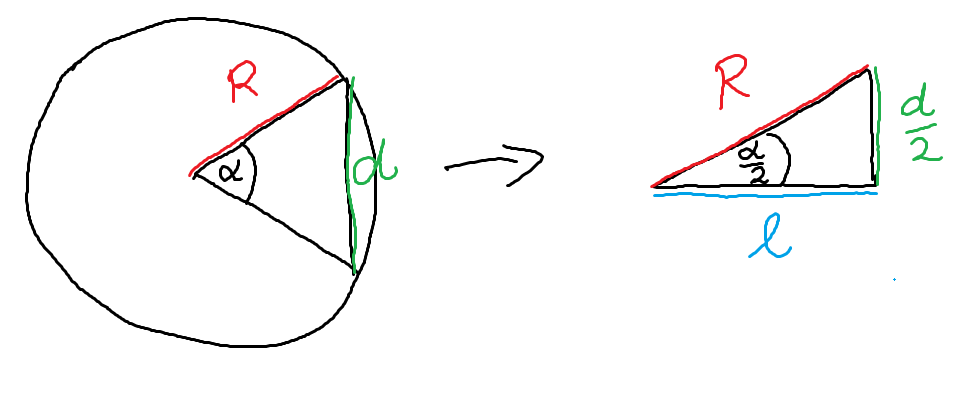
\includegraphics[scale=.5]{./images/kuzel4.png}
    \label{fig:enter-label}
\end{figure}
Trojúhelníček má stranu $d$ v podstavě válce. Když si domyslíme kruh o poloměru $R,$ do kterého je vepsaný pravidelný $n$-úhelník (=podstava jehlanu), úsečka $d$ je sečna tohoto kruhu a odpovídá jí úhel $\alpha.$ Takových úseček se tam má vlézt $n$, proto $\alpha = \frac{2\pi}{n}.$ Z trojúhelníčku $R,l,\frac{d}{2}$ máme
\begin{equation*}
    d = 2R\cdot \sin\frac{\alpha}{2}, \ \ \ l=R\cdot \cos\frac{\alpha}{2}
\end{equation*}
(sinus = protilehlá ku přeponě, koninus = přilehlá ku přeponě).
\begin{figure}[h]
    \centering
    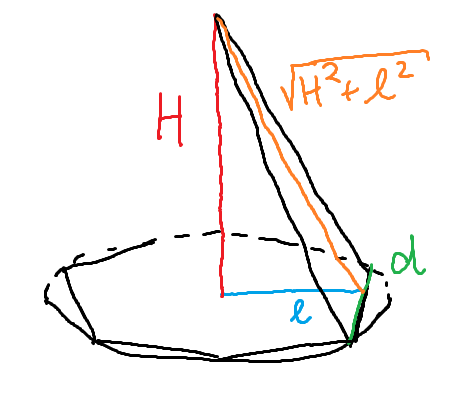
\includegraphics[scale=.5]{./images/kuzel5.png}
    \label{fig:enter-label}
\end{figure}
Základna trojúhelníku je $d,$ výška $\sqrt{H^2+l^2}.$ Obsah je tedy
\begin{align*}
    T_n &= \frac{1}{2}\cdot d \cdot \sqrt{H^2+l^2} = R\cdot\sin\frac{\alpha}{2}\cdot  \displaystyle\sqrt{H^2+R^2\cdot\cos^2\frac{\alpha}{2}} \\
    &= R\cdot \sin\frac{\pi}{n}\cdot \displaystyle\sqrt{H^2+R^2\cdot \cos^2\frac{\pi}{n}}
\end{align*}

\vspace{1cm}
\par \textbf{KROK 2:} 
\begin{equation*}
    S = \lim_{n\to \infty} n\cdot T_n = \lim_{n\to \infty} n\cdot R\cdot \sin\frac{\pi}{n}\cdot \displaystyle\sqrt{H^2+R^2\cdot \cos^2\frac{\pi}{n}} = ... = \pi R \sqrt{H^2+R^2}
\end{equation*}

\subsubsection*{3: \uv{normálová derivace objemu}}
\par \textbf{Domněnka (neověřená):} Pokud povrch tělesa rozšíříme o stejné $\Delta d$ všude ve směru normály (=kolmici k ploše), nové \uv{nafouklé} těleso bude mít objem o 
\begin{equation*}
    \Delta V = S\cdot \Delta d + o(\Delta d)
\end{equation*}
větší, kde $S$ byl původní povrch tělesa. Tedy $S = \displaystyle\lim_{\Delta d \to 0} \frac{\Delta V}{\Delta d}.$

\vspace{.5cm}
\par \textbf{Poznámka:} \uv{o} notace tady znamená, že $o(\Delta d)$ je nějaká funkce splňující
\begin{equation*}
    \lim_{\Delta d \to 0}\frac{o(\Delta d)}{\Delta d} = 0.
\end{equation*}
Typicky se tam může objevit $(\Delta d)^2, (\Delta d)^3$ atd.

\vspace{.5cm}
\textbf{Příklad: Koule.} Objem koule o poloměru $R$ je $\frac{4}{3}\pi R^3.$ Když zvětšíme poloměr z $R$ na $R+\Delta R,$ je to přesně případ popsaný v domněnce (nafoukli jsme kouli všude ve směru normály, tj. směrem od středu, a všude o stejné $\Delta R.$) Nový objem je
\begin{align*}
    \frac{4}{3}\pi (R+\Delta R)^3 &= \frac{4}{3}\pi (R^3 + 3R^2\cdot \Delta R + 3R\cdot (\Delta R)^2 + (\Delta R)^3) \\
    &= \frac{4}{3}\pi (R^3 + 3R^2\cdot \Delta R + o(\Delta R)) = \frac{4}{3}\pi R^3 + 4\pi R^2 \Delta R + o(\Delta R)
\end{align*}
Změna objemu je tedy až na zanedbatelný člen $4\pi R^2 \Delta R,$ což souhlasí s tím, že povrch koule je $4\pi R^2.$ Jednoduše na toto dojdeme, pokud si spočítáme
\begin{equation*}
    \frac{d}{dR}\left(\frac{4}{3}\pi R^3 \right) = 4\pi R^2.
\end{equation*}
\par \textbf{Strategie pro kužel:} 
\begin{itemize}
    \item Objem kužele je $\frac{1}{3}\pi R^2 H.$
    \item Podstavu kužele zvětšíme o $\Delta R,$ výšku o $\Delta H$ tak, aby měl kužel \uv{stejný tvar}, tj. aby odpovídající povrchové přímky byly rovnoběžné. To zaručí, že kolmá vzdálenost ploch (to je naše $\Delta d$ v domněnce) je všude stejná. Tuto vzdálenost musíme samozřejmě spočítat.
    \item Vyjádříme $\Delta H, \Delta d$ pomocí $\Delta R,$ a výsledek bude $S=\lim_{\Delta R \to 0} \frac{\Delta V}{\Delta d}$ (stejný, jako kdybychom počítali derivaci. Takto je ovšem výpočet příjemnější a vyhneme se nešikovnému zápisu $S=\frac{dV}{dd}.$)
\end{itemize}

\begin{figure}[h]
    \centering
    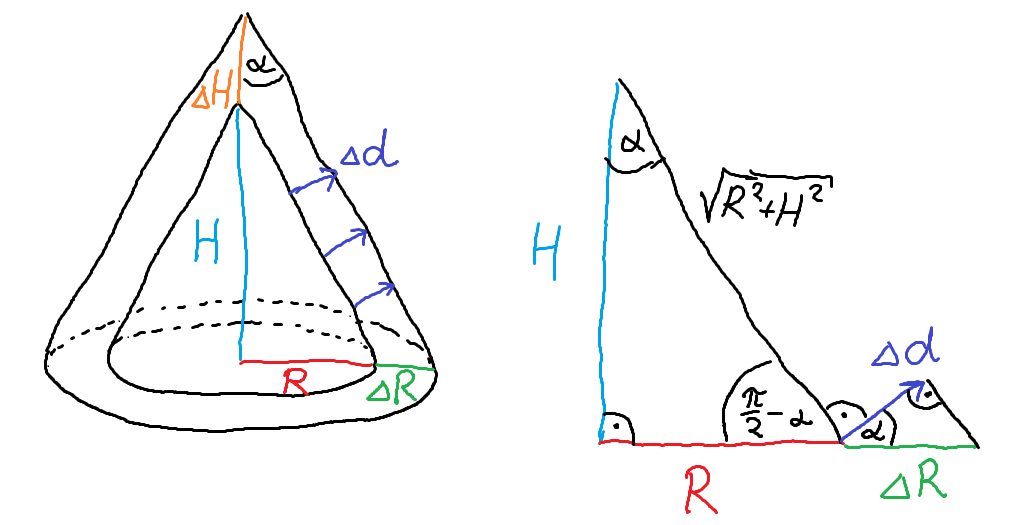
\includegraphics[scale=.5]{./images/kuzel6.png}
    \label{fig:enter-label}
\end{figure}

Aby měly kužel stejný tvar, musí platit
\begin{equation*}
    \frac{H+\Delta H}{R+\Delta R} = \frac{H}{R} \ \Rightarrow \ \Delta H = \frac{H}{R}\Delta R
\end{equation*}
Protože se $\Delta R, \Delta H$ liší jen o multiplikativní konstantu, platí $o(\Delta R) = o(\Delta H).$ Ve výpočtu změny objemu budeme tyto zanedbatelné členy rovnou psát společně jako $o(\Delta R).$ Jedná se o členy typu $(\Delta R)^2, (\Delta R)^2 \cdot \Delta H, (\Delta H)^2$ (vše, kde je \uv{víc než jedna delta.})

\begin{align*}
    \Delta V &= \frac{1}{3}\pi (R+\Delta R)^2(H+\Delta H) - \frac{1}{3}\pi R^2\cdot H \\
    &= \frac{1}{3} \pi (R^2+2R\cdot \Delta R)(H+\Delta H) - \frac{1}{3}\pi R^2 \cdot H + o(\Delta R) \\
    &= \frac{1}{3} \pi (R^2\cdot H+2R\cdot \Delta R \cdot H + R^2\cdot \Delta H) - \frac{1}{3}\pi R^2 \cdot H + o(\Delta R) \\
    &= \frac{1}{3} \pi (2R\cdot \Delta R \cdot H + R^2\cdot \Delta H) + o(\Delta R) \\
    &= \frac{1}{3} \pi (3\Delta R \cdot H) + o(\Delta R) = \pi \cdot H \cdot \Delta R + o(\Delta R)
\end{align*}
Z předposledního na poslední řádek jsem využil vztah mezi $\Delta H, \Delta R.$ 

\vspace{.5cm}
\par Ještě zbývá spočítat $\Delta d.$ Vidíme, že normálový vektor o délce $\Delta d$ s podstavou kuželu svírá úhel $\alpha,$ tedy stejný úhel jako svírají povrchové přímky pláště s osou (k tomu dospějeme přes úhel $\frac{\pi}{2}-\alpha$ na obrázku, součet ostrých úhlů v pravoúhlém trojúhelníku je $\frac{\pi}{2}$ a součet tří úhlů tvořících přímý úhel je $\pi.$) Využitím podobnosti trojúhelníků:
\begin{equation*}
    \Delta d = \Delta R \cdot \cos\alpha = \Delta R \cdot \frac{H}{\sqrt{R^2+H^2}}
\end{equation*}
Konečně tedy
\begin{equation*}
    S = \lim_{\Delta R \to 0} \frac{\Delta V}{\Delta d} = \lim_{\Delta R\to 0} \frac{\pi \cdot H \cdot \Delta R + o(\Delta R)}{\Delta R \cdot \frac{H}{\sqrt{R^2+H^2}}} = \pi R \sqrt{R^2+H^2}
\end{equation*}
\vspace*{1cm}

\par \textbf{Poznámka:} Z obrázku se může zdát, že jsme zanedbali nově vzniklou plochu u podstavy a \uv{v čepičce}. 
\vspace{1cm}
\begin{figure}[h]
    \centering
    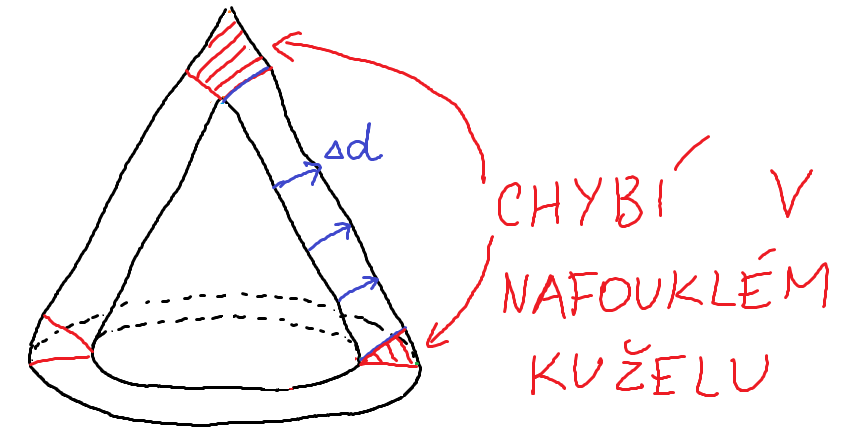
\includegraphics[scale=.5]{./images/kuzel7.png}
    \label{fig:enter-label}
\end{figure}
Jde ale vidět, že zanedbané části jsou řádově $\Delta d \cdot \Delta H,$ resp. $\Delta d \cdot \Delta R,$ tedy typu $o(\Delta R)$ a konečný výsledek neovlivní.

%TODO: DODELAT NEBO SMAZAT?
\end{document}

